%%%%%%%%%%%%%%%%%%%%%%%%%%%%%%%%%%%%%%%%%%%%%%%%%%%%%%%%%%%%%%%%%%%%%%
% Lớp 12 | Phương trình mặt phẳng, đường thẳng, mặt cầu | Phương trình mặt phẳng
% Dạng 2H5?1-4: Vị trí tương đối giữa hai mặt phẳng (song song, vuông góc)
% Số câu: 41  (sinh tự động bởi tach_cau.py; từ nay thầy sửa trực tiếp file này)
%%%%%%%%%%%%%%%%%%%%%%%%%%%%%%%%%%%%%%%%%%%%%%%%%%%%%%%%%%%%%%%%%%%%%%

%%%%%%%%%%%%%%%% TRẮC NGHIỆM 4 PHƯƠNG ÁN %%%%%%%%%%%%%%%%

% nguồn: Phan1_Lop_12_Hinh_hoc_Chuong_5
\begin{ex}%[2H5N1-4]%[ma:c25d82f8]
	Trong không gian $Oxyz$, mặt phẳng $(P)$ có phương trình $x-y+2z-1=0$  song song với mặt phẳng nào trong các mặt phẳng sau đây?
	 \choice
		{$x+y+2z+3=0$} 
		{$2x-2y+4z-2=0$} 
		 {$x+2y-z=0$}
		{\True  $x-y+2z+6=0$}
	 \loigiai{
		Xét mặt phẳng có phương trình $x-y+2z+6=0$.\\ 
		Ta thấy $\dfrac{1}{1}=\dfrac{-1}{-1}=\dfrac{2}{2}\neq \dfrac{-1}{6}$ nên hai mặt phẳng  song song.
	 }
\end{ex}

% nguồn: Phan1_Lop_12_Hinh_hoc_Chuong_5
\begin{ex}%[2H5N1-4]%[ma:43f4468b]
	Trong không gian hệ tọa độ $Oxyz$, cho điểm $A(1;1;1)$ và hai mặt phẳng $(P)\colon 2x - y + 3z - 1 = 0$, $(Q): y = 0$. Viết phương trình mặt phẳng $(R)$ chứa $A$, vuông góc với cả hai mặt phẳng $(P)$ và  $(Q)$.
	\choice 
		{$3x - y + 2z - 4  = 0$}
		{$3x - y +  2z - 2 = 0$}
		{$3x - 2z =  0$}
		{\True $3x - 2z - 1 =  0$}
	\loigiai{ 
		$(P)\colon 2x - y + 3z - 1 = 0$  có vectơ pháp tuyến $\overrightarrow{n_{(P)}} = (2;-1;3)$.\\
		$(Q)\colon y = 0$ có vectơ  pháp tuyến $\overrightarrow{n_{(Q)}} = (0;1;0)$.\\
		Do mặt phẳng $(R)$ vuông góc với cả hai mặt phẳng $(P)$ và  $(Q)$ nên có vectơ pháp tuyến $$\overrightarrow{n_{(R)}} = [\overrightarrow{n_{(P)}}, \overrightarrow{n_{(Q)}}] = (-3;0;2).$$
		Vậy phương trình mặt phẳng $(R)$ là $-3(x - 1) + 0(y -  1) + 2(z - 1) = 0 \Leftrightarrow 3x - 2z - 1 = 0$.
	} 
\end{ex}

% nguồn: Phan1_Lop_12_Hinh_hoc_Chuong_5
\begin{ex}%[2H5N1-4]%[ma:ec90f3a2]
	Trong không gian hệ tọa độ $Oxyz$, mặt phẳng đi qua ba  điểm $A(2;3;5)$, $B(3;2;4)$ và $C(4;1;2)$ có phương trình là
	 \choice
		{$3x - y - 2z - 4  = 0$}
		{\True $x + y - 5 = 0$} 
		{$y -  z + 2 = 0$}
		 {$2x + y - 7 = 0$}
	\loigiai{ 
		Ta có $\overrightarrow{AB}  = (1;-1;-1)$, $\overrightarrow{AC} = (2;-2;-3)$ suy ra $\overrightarrow{n} = [\overrightarrow{AB}, \overrightarrow{AC}] = (1;1;0)$.\\
		Vì $\overrightarrow{AB}$, $\overrightarrow{AC}$ không cùng phương (do $1/2 \neq -1/-3$) nên $\overrightarrow{n} = [\overrightarrow{AB}, \overrightarrow{AC}]$ làm một vectơ pháp  tuyến.\\
		Vì $(ABC)$ đi qua $A(2;3;5)$ nên phương trình  của $(ABC)$ là
		$$1(x - 2) + 1(y - 3)  + 0(z - 5) = 0 \Leftrightarrow x + y - 5 = 0.$$
	} 
\end{ex}

% nguồn: Phan1_Lop_12_Hinh_hoc_Chuong_5
\begin{ex}%[2H5N1-4]%[ma:03ded065]
	Trong không gian với hệ tọa độ $Oxyz$, mặt phẳng $(P)\colon 2x + y + z - 2 = 0$ song song với mặt phẳng nào  dưới đây?
	 \choice
		{$x +  \dfrac{1}{2}y - \dfrac{1}{2}z - 1 = 0$}
		{$x - y  - z - 0 = 0$}
		{\True $4x + 2y + 2z +  4 = 0$}
		{$2x + y + z - 2  = 0$}
	\loigiai{ 
		Xét $(P)$ và $(Q_1)\colon x + \dfrac{1}{2}y  - \dfrac{1}{2}z - 1 = 0$ có $\dfrac{2}{1} \neq \dfrac{1}{-1} \neq \dfrac{1}{-1} \Rightarrow (P)$ không song song với $(Q_1)$.\\
		Xét $(P)$ và $(Q_2)\colon x - y - z - 0 = 0$ có  $\dfrac{2}{1} \neq \dfrac{1}{-1} = \dfrac{1}{-1} \Rightarrow (P)$ không song song với $(Q_2)$.\\
		Xét $(P)$ và $(Q_3)\colon 4x + 2y  + 2z + 4 = 0$ có $\dfrac{2}{4} = \dfrac{1}{2} = \dfrac{1}{2} \neq \dfrac{-2}{4} \Rightarrow (P)$ song song với $(Q_3)$.\\
		Xét $(P)$ và $(Q_4)\colon 2x + y + z - 2 = 0$ có $\dfrac{2}{2} = \dfrac{1}{1} = \dfrac{1}{1} = \dfrac{-2}{-2} \Rightarrow (P)$ trùng với $(Q_4)$. 
	 }
\end{ex}

% nguồn: Phan1_Lop_12_Hinh_hoc_Chuong_5
\begin{ex}%[2H5N1-4]%[ma:3e1ed2b5]
	Trong không gian hệ tọa độ $Oxyz$, cho hai điểm  $A(4;0;1)$ và $B(-2;2;3)$. Phương trình nào dưới đây là phương trình mặt phẳng trung trực của đoạn thẳng $AB$?
	\choice 
		{$3x + y + z - 6  = 0$}
		{$6x - 2y - 2z - 1 =  0$}
		{$3x - y - z  + 1 = 0$}
		{\True  $3x - y - z = 0$}
	\loigiai{ 
		Gọi $I$  là trung điểm của đoạn thẳng $AB$, suy ra $I(1;1;2)$.\\
		Gọi $(\alpha)$ là mặt phẳng trung trực của  đoạn thẳng $AB$.\\
		$(\alpha)$ đi qua $I(1;1;2)$ và nhận $\overrightarrow{AB} = (-6;2;2)$ làm vectơ  pháp tuyến.\\
		Phương trình mặt phẳng $(\alpha)$ là $-6(x - 1) + 2(y - 1) + 2(z - 2) = 0 \Rightarrow 3x  - y - z = 0$.
	} 
\end{ex}

% nguồn: Phan1_Lop_12_Hinh_hoc_Chuong_5
\begin{ex}%[2H5N1-4]%[ma:de4daae4]
	Trong không gian với hệ tọa độ $Oxyz$, cho điểm $A(2;-1;-3)$  và mặt phẳng $(P)\colon 3x - 2y + 4z - 5 = 0$. Gọi $(Q)$ là mặt phẳng đi qua $A$ và song song với mặt phẳng $(P)$. Mặt phẳng $(Q)$ có phương trình là:
	 \choice
		{$3x -  2y + 4z - 4 = 0$}
		{\True $3x - 2y + 4z + 4 =  0$}
		{$3x - 2y + 4z + 5 =  0$}
		{$3x  - 2y + 4z + 8 = 0$}
	 \loigiai{
		Mặt phẳng  $(P)\colon 3x - 2y + 4z - 5 = 0$ có một vectơ pháp tuyến là $\overrightarrow{n}_{(P)} = (3;-2;4)$.\\
		Do $(Q)$ song song với $(P)$  nên $(Q)$ có vectơ pháp tuyến là $\overrightarrow{n}_{(Q)} = (3;-2;4)$.\\
		Phương trình mặt phẳng $(Q)$ là $3(x  - 2) - 2(y + 1) + 4(z + 3) = 0 \Leftrightarrow 3x - 2y + 4z + 4 = 0$.
	} 
\end{ex}

% nguồn: Phan1_Lop_12_Hinh_hoc_Chuong_5
\begin{ex}%[2H5N1-4]%[ma:f316fe26]
	Trong không gian với hệ tọa độ $Oxyz$, cho mặt phẳng $(P)$ có phương trình: $mx + (m - 1)y + z - 10 = 0$ và mặt phẳng $(Q)\colon 2x + y - 2z + 3 = 0$. Với giá trị nào của dưới đây của $m$ thì $(P)$ và $(Q)$ vuông góc với  nhau
	 \choice
		{$m = -2$} 
		{\True  $m = 1$}
		{$m = 2$} 
		{$m = -1$} 
	\loigiai{ 
		Mặt phẳng $(P)\colon mx + (m - 1)y  + z - 10 = 0$ có vectơ pháp tuyến $\overrightarrow{n_{(P)}} = (m; m - 1; 1)$.\\
		Mặt phẳng $(Q): 2x + y - 2z + 3 = 0$ có vectơ pháp tuyến  $\overrightarrow{n_{(Q)}} = (2; 1; -2)$.\\
		Hai mặt phẳng $(P)$ và $(Q)$ vuông  góc
		\begin{eqnarray*}
			&&\Leftrightarrow \overrightarrow{n_{(P)}} \perp \overrightarrow{n_{(Q)}}  \\
			&&\Leftrightarrow \overrightarrow{n_{(P)}} \cdot \overrightarrow{n_{(Q)}}  = 0 \\
			&&\Leftrightarrow m \cdot 2 + (m - 1) \cdot 1 + 1 \cdot (-2) = 0\\ 
			&&\Leftrightarrow  m=1.
		\end{eqnarray*}
	 }
\end{ex}

% nguồn: Phan1_Lop_12_Hinh_hoc_Chuong_5
\begin{ex}%[2H5N1-4]%[ma:e6902c5f]
	Trong  không gian $Oxyz$, mặt phẳng $(P)\colon x-y+z+1=0$ vuông góc với mặt phẳng nào trong các mặt phẳng sau đây?
	\choice 
		{$x+y+z+1=0$} 
		 {$x-2 y+z+1=0$}
		 {\True $x+2 y+z=0$}
		 {$x-y+z+1=0$}
	 \loigiai{
		$(P)\colon x-y+z+1=0$ có vectơ pháp tuyến  $\overrightarrow{n}_P=(1;-1;1)$.\\
		 Xét $x+2 y+z=0$ có vectơ pháp tuyến $\overrightarrow{n}=(1;2;1)$.\\
		Ta có  $\overrightarrow{n}_P\cdot \overrightarrow{n}=1-2+1=0$ nên $(P)$ vuông góc với mặt phẳng có phương trình $x+2 y+z=0$.
	 }
\end{ex}

% nguồn: Phan1_Lop_12_Hinh_hoc_Chuong_5
\begin{ex}%[2H5H1-4]%[ma:950a4d80]
	Trong không gian với hệ tọa độ $Oxyz$, phương trình mặt phẳng $(P)$ đi qua hai điểm $A(2;-1;0)$ và $B(1;1;2)$ và vuông góc với mặt phẳng $(Q):  x + y + z - 3 = 0$ là
	 \choice
		 {$2x + 4y - 3z - 8 = 0$}
		{\True $2x  - 4y + 3z - 8 = 0$}
		{$2x + 4y - 3z  + 8 = 0$}
		{$2x - 4y -  3z = 0$}
	 \loigiai{
		Mặt phẳng  $(Q)$ có một vectơ pháp tuyến $\overrightarrow{n_{(Q)}} = (1;1;2)$.\\
		Mặt phẳng $(P)$ đi qua hai điểm $A(2;-1;0)$, $B(1;1;2)$ và vuông góc với mặt phẳng $(Q)$ nên có cặp vectơ chỉ phương là  $\overrightarrow{AB} = (-1;2;2)$ và $\overrightarrow{n_{(Q)}} = (1;1;2)$.\\
		Do đó  $(P)$ có vectơ pháp tuyến là
		$\overrightarrow{n}_{(P)} = [\overrightarrow{AB}, \overrightarrow{n_{(Q)}}] =  (2;-4;3)$.\\
		Mặt phẳng $(P)$ đi  qua điểm $A(2;-1;0)$ và nhận $\overrightarrow{n}_{(P)} = (2;-4;3)$ làm vectơ pháp tuyến nên có phương trình là
		$$2(x - 2) - 4(y + 1) + 3(z - 0) = 0 \Leftrightarrow 2x - 4y + 3z - 8 = 0.$$ 
	 }
\end{ex}

% nguồn: Phan1_Lop_12_Hinh_hoc_Chuong_5
\begin{ex}%[2H5H1-4]%[ma:fdbe9c7f]
	Trong không gian $Oxyz$, mặt phẳng nào dưới đây vuông góc  với mặt phẳng $(P) \colon 4x-14y-z+4=0$
	 \choice
		 {\True $3x+y-2z+15=0$}
		 {$4x-14y-z=0$}
		{$3x+y+2z+15=0$} 
		{$x+y-12z+1=0$} 
	\loigiai{ 
		Mặt phẳng vuông góc với $(P)$ thì vectơ pháp tuyến của 2 mặt phẳng sẽ vuông góc với nhau hoặc tích  vô hướng bằng không.\\
		Ta có $3x+y-2z+15=0$ vuông góc với $(P)$ vì $(P)$ có $1$ vectơ pháp tuyến~là $\vec{n}=(3;1;-2)$ thỏa mãn $\vec{n}_{(P)}  \cdot \vec{n}_{(P)}=3\cdot4-14+2=0$.
	} 
\end{ex}

% nguồn: Phan1_Lop_12_Hinh_hoc_Chuong_5
\begin{ex}%[2H5H1-4]%[ma:88a142b9]
	Trong không gian với hệ tọa độ $Oxyz$, cho điểm $A(2;3;5)$. Viết phương trình mặt phẳng $(\alpha)$ đi  qua $A$ và chứa trục $Ox$.
	\choice 
		{$(\alpha): 5y + 3z =  0$}
		{$(\alpha): 3y + 5z = 0$} 
		{$(\alpha): 3y - 5z  = 0$}
		{\True  $(\alpha): 5y - 3z = 0$}
	\loigiai{ 
		Mặt phẳng $(\alpha)$ có dạng $By + Cz = 0$ và  $A \in (\alpha) \Rightarrow 3B + 5C = 0 \Rightarrow 3B = -5C$.\\
		Chọn  $B = 5 \Rightarrow C = -3$.\\
		Vậy $(\alpha)\colon  5y - 3z = 0$.
	 }
\end{ex}

% nguồn: Phan1_Lop_12_Hinh_hoc_Chuong_5
\begin{ex}%[2H5H1-4]%[ma:851df70a]
	Trong không gian với hệ tọa độ  $Oxyz$, mặt phẳng đi qua điểm $A(2;-3;-2)$ và song song với mặt phẳng $(\alpha)\colon 2x - y + 3z - 3 = 0$ có phương trình là
	\choice 
		 {$2x - y + 3z = 0$}
		{\True $2x - y +  3z - 1 = 0$}
		{$2x - 3y  - 2z = 0$}
		{$2x - 3y -  2z - 1 = 0$}
	 \loigiai{
		Gọi $(P)$ là mặt phẳng cần tìm. Do $(P)\parallel(\alpha) \Rightarrow \overrightarrow{n_{(P)}} = \overrightarrow{n_{(\alpha)}} = (2;-1;3)$.\\ 
		Vì $(P)$ đi qua điểm $A$ nên $(P)\colon 2(x - 2) - 1(y + 3) + 3(z  + 2) = 0 \Rightarrow (P)\colon 2x - y + 3z - 1 = 0$.
	 }
\end{ex}

% nguồn: Phan1_Lop_12_Hinh_hoc_Chuong_5
\begin{ex}%[2H5H1-4]%[ma:3e7268fc]
	cau14 
	Trong không gian với hệ tọa độ $Oxyz$, cho điểm $A(2;-4;5)$. Viết phương trình mặt phẳng $(\alpha)$ đi qua $A$ và chứa trục $Oz$. 
	\choice 
		 {$ x - 2y = 0$}
		{$x + 2y  = 0$}
		{$2x - y =  0$}
		{\True $2x  + y = 0$}
	 \loigiai{
		Mặt phẳng $(\alpha)$ có dạng $Ax + By = 0$ và $A \in (\alpha) \Rightarrow 2A - 4B  = 0 \Rightarrow A = 2B$.\\
		Chọn  $A = 2 \Rightarrow B = 1 \Rightarrow (\alpha)\colon 2x + y = 0$.
	 }
\end{ex}

% nguồn: Phan1_Lop_12_Hinh_hoc_Chuong_5
\begin{ex}%[2H5H1-4]%[ma:6ae42ae5]
	Trong không gian với hệ tọa độ $Oxyz$, cho điểm $A(-3;1;2)$. Viết phương trình mặt phẳng $(\alpha)$  đi qua $A$ và chứa trục $Oy$.
	 \choice
		{$(\alpha): 2x -  3z = 0$}
		{$(\alpha): 3x + 2z = 0$} 
		{$(\alpha): 3x - 2z = 0$} 
		{\True $(\alpha)\colon 2x  + 3z = 0$}
	\loigiai{ 
		Mặt phẳng $(\alpha)$ có dạng $Ax + Cz = 0$ và $A \in (\alpha) \Rightarrow -3A + 2C = 0 \Rightarrow 3A =  2C$.\\
		Chọn $A = 2 \Rightarrow C = 3 \Rightarrow  (\alpha)\colon 2x + 3z = 0$.
	 }
\end{ex}

% nguồn: Phan1_Lop_12_Hinh_hoc_Chuong_5
\begin{ex}%[2H5H1-4]%[ma:7ad181ff]
	Trong không gian với  hệ tọa độ $Oxyz$, cho hai điểm $A(-1;2;0)$ và $B(3;0;2)$. Mặt phẳng trung trực của đoạn thẳng $AB$ có phương trình là
	 \choice
		{$x + y +  z - 3 = 0$}
		{$2x - y +  z + 2 = 0$}
		{$2x + y + z - 4 =  0$}
		{\True $2x - y + z - 2 =  0$}
	 \loigiai{
		Gọi  $I$ là trung điểm của đoạn thẳng $AB$. Suy ra $I(1;1;1)$ và $\overrightarrow{AB} = (4;-2;2)$.\\
		Phương trình mặt phẳng trung trực của đoạn thẳng $AB$ đi qua trung điểm $I$ của $AB$ và nhận $\overrightarrow{AB}$ làm vectơ pháp tuyến nên có phương trình  là
		$$4(x - 1) - 2(y - 1) + 2(z  - 1) = 0 \Leftrightarrow 2x - y + z - 2 = 0.$$
	} 
\end{ex}

% nguồn: Phan1_Lop_12_Hinh_hoc_Chuong_5
\begin{ex}%[2H5H1-4]%[ma:728c94c0]
	Trong không gian $Oxyz$, cho mặt phẳng $(P)\colon 6x + 8y + 10z - 4  = 0$. Mặt phẳng nào dưới đây song song với $(P)$?
	 \choice
		{\True $3x + 4y + 5z +  1 = 0$}
		{$x + y - z - 4 =  0$}
		 {$3x + 4y + 5z - 2 = 0$}
		 {$6x + 8y - 10z - 4 = 0$}
	\loigiai{ 
		Mặt phẳng $3x + 4y + 5z + 1 = 0$  song song với $(P)\colon 6x + 8y + 10z - 4 = 0$.
	 }
\end{ex}

% nguồn: Phan1_Lop_12_Hinh_hoc_Chuong_5
\begin{ex}%[2H5H1-4]%[ma:7d921295]
	Trong không gian với  hệ tọa độ $Oxyz$, mặt phẳng đi qua điểm $A(2;-3;-2)$ và song song với mặt phẳng $(Oyz)$ có phương trình là
	 \choice
		{$3y - 2z  = 0$}
		 {$x + 2 = 0$}
		{\True $x - 2  = 0$}
		 {$3y + 2z = 0$}
	 \loigiai{
		Gọi $(P)$ là mặt  phẳng cần tìm.\\
		Do $(P)\parallel(Oyz) \Rightarrow \overrightarrow{n_{(P)}}  = \overrightarrow{i} = (1;0;0)$.\\
		Và $(P)$ đi qua điểm $A \Rightarrow (P)\colon 1\cdot(x  - 2) + 0\cdot(y + 3) + 0\cdot(z + 2) = 0 \Rightarrow (P)\colon x - 2 = 0$.
	 }
\end{ex}

% nguồn: Phan1_Lop_12_Hinh_hoc_Chuong_5
\begin{ex}%[2H5H1-4]%[ma:cd75d32e]
	Trong không gian với hệ tọa độ $Oxyz$, cho hai mặt phẳng $(\alpha)\colon 3x - 2y + 2z + 7 = 0$ và $(\beta)\colon 5x - 4y + 3z + 1 = 0$. Phương trình mặt phẳng đi qua gốc tọa độ $O$ đồng  thời vuông góc với cả $(\alpha)$ và $(\beta)$ là
	 \choice
		{\True $2x + y -  2z = 0$}
		{$x +  y + z + 3 = 0$}
		{$-2x + z  + 6 = 0$}
		{$-2x + z  - 6 = 0$}
	\loigiai{ 
		Vectơ pháp tuyến của hai mặt phẳng lần lượt là $\overrightarrow{n_{(\alpha)}} = (3;-2;2)$, $\overrightarrow{n_{(\beta)}} =  (5;-4;3)$.\\
		Vì mặt phẳng $(P)$ đồng thời vuông góc với cả $(\alpha)$ và $(\beta)$ nên $(P)$ nhận  hai vectơ\break $\overrightarrow{n_{(\alpha)}} = (3;-2;2)$, $\overrightarrow{n_{(\beta)}} = (5;-4;3)$ làm cặp vectơ chỉ phương suy ra $(P)$ có vectơ pháp tuyến là
		$\overrightarrow{n} = [\overrightarrow{n_{(\alpha)}}; \overrightarrow{n_{(\beta)}}]  = (2;1;-2)$.\\
		Mặt phẳng $(P)$ đi qua gốc tọa độ $O$ nên $(P)\colon 2x + y - 2z =  0$.
	} 
\end{ex}

% nguồn: Phan1_Lop_12_Hinh_hoc_Chuong_5
\begin{ex}%[2H5H1-4]%[ma:d620b541]
	Trong không gian với hệ tọa độ $Oxyz$, cho bốn điểm $A(1;0;1)$, $C(3;1;1)$, $D(4;1;1)$, $B(-1;2;2)$. Viết phương  trình mặt phẳng đi qua hai điểm $A, B$ và song song với $CD$.
	\choice 
		{\True $y -  2z + 2 = 0$}
		{$x - 2z + 2  = 0$}
		{$x - y + 2z =  0$}
		{$x - 2y + 2 =  0$}
	\loigiai{ 
		Gọi $(P)$ là mặt  phẳng cần tìm.\\
		Vì $(P)$ đi qua hai điểm $A$, $B$ và song song với  $CD$ nên $(P)$ nhận hai vectơ $\overrightarrow{AB} = (-2;2;1)$, $\overrightarrow{CD} = (1;0;0)$ làm cặp vectơ chỉ phương.\\
		Suy ra $(P)$ có  vectơ pháp tuyến là
		$\overrightarrow{n} = \left[\overrightarrow{CD}, \overrightarrow{AB}\right] = (0;-1;2)$.\\ 
		Phương trình mặt phẳng $(P)$ là $0(x - 1) - 1(y - 0) + 2(z - 1) = 0$ hay $y - 2z +  2 = 0$.
	} 
\end{ex}

% nguồn: Phan1_Lop_12_Hinh_hoc_Chuong_5
\begin{ex}%[2H5H1-4]%[ma:23a0cda7]
	Trong không gian với hệ tọa độ $Oxyz$, cho $A(1;2;-1)$, $B(-1;0;1)$ và mặt phẳng $(P)\colon x + 2y - z + 1 = 0$. Viết phương trình mặt phẳng $(Q)$ qua $A,  B$ và vuông góc với $(P)$.
	\choice 
		{$2x -  y + 3 = 0$}
		 {\True $x + z = 0$}
		{$-x + y  + z = 0$}
		{$3x - y  + z = 0$}
	 \loigiai{
		Ta có $\overrightarrow{AB}  = (-2;-2;2) = -2(1;1;-1)$, và $\overrightarrow{n_{(P)}} = (1;2;-1)$.\\
		Vì mặt phẳng $(Q)$ qua $A$, $B$ và vuông góc với $(P)$  nên $(Q)$ nhận vectơ $\overrightarrow{u} = (1;1;-1)$ và $\overrightarrow{n_{P}} = (1;2;-1)$ làm cặp vectơ chỉ phương.\\
		 Suy ra $(Q)$ có vectơ pháp tuyến là
		$\overrightarrow{n_{(Q)}} = [\overrightarrow{u}, \overrightarrow{n_{(P)}}]  = (1;0;1)$.\\
		 Mặt phẳng $(Q)$ qua $A \Rightarrow (Q)\colon x + z = 0$.
	} 
\end{ex}

% nguồn: Phan1_Lop_12_Hinh_hoc_Chuong_5
\begin{ex}%[2H5H1-4]%[ma:0f7e3f02]
	Trong không gian với hệ tọa độ $Oxyz$, mặt phẳng chứa trục $Ox$ và vuông góc với mặt phẳng $(\alpha)\colon 2x-3y+4z-5=0$ có  phương trình là
	\choice 
		 {$2x-3y+4z-5=0$}
		{$4y-3z=0$} 
		{$3x+4y=0$} 
		{\True $4y+3z=0$} 
	\loigiai{Trục $Ox$ có vectơ chỉ phương $\overrightarrow{i}=(1;0;0)$ và mặt phẳng  $(\alpha)$ có vectơ pháp tuyến $\overrightarrow{n}=(2;-3;4)$.\\
		Mặt phẳng $(P)$  chứa trục $Ox$ và vuông góc với $(\alpha)$ khi và chỉ khi $(\alpha)$ đi qua điểm $O(0;0;0)$ và có vectơ pháp tuyến là $\overrightarrow{m}=[\overrightarrow{i},\overrightarrow{n}]=(0;-4;-3).$\\
		 Vậy $(P)$ có phương trình là
	$$0(x-0)-4(y-0)-3(z-0)=0\Leftrightarrow 4y+3z=0.$$} 
\end{ex}

% nguồn: Phan1_Lop_12_Hinh_hoc_Chuong_5
\begin{ex}%[2H5H1-4]%[ma:f8f5129c]
	Trong không gian với hệ tọa độ  $Oxyz$, mặt phẳng đi qua điểm $A(2;-3;-2)$ và song song với mặt phẳng $(Oxz)$ có phương trình là
	 \choice
		{$x  + z = 0$}
		{\True $y + 3  = 0$}
		{$y - 3 = 0$} 
		 {$x - z = 0$}
	\loigiai{ 
		Gọi $(P)$  là mặt phẳng cần tìm.\\
		 Do $(P)\parallel (Oxz) \Rightarrow \overrightarrow{n_{(P)}} = \overrightarrow{j} = (0;1;0)$.\\
		Và $(P)$ đi qua điểm $A \Rightarrow (P)\colon 0(x - 2) + 1(y + 3) + 0(z  + 2) = 0 \Rightarrow (P)\colon y + 3 = 0$.
	 }
\end{ex}

% nguồn: Phan1_Lop_12_Hinh_hoc_Chuong_5
\begin{ex}%[2H5H1-4]%[ma:fc4d2822]
	Trong không  gian với hệ tọa độ $Oxyz$, mặt phẳng đi qua điểm $A(2;-3;-2)$ và song song với mặt phẳng $(Oxy)$ có phương trình là
	 \choice
		{\True $z +2=0$} 
		 {$z-2=0$}
		{$2x-3y=0$} 
		 {$2x-3y-2=0$}
	 \loigiai{
		Gọi $(P)$  là mặt phẳng cần tìm.\\
		Do $(P)\parallel (Oxy) \Rightarrow \overrightarrow{n_{(P)}} =  \overrightarrow{k} = (0;0;1)$.\\
		Và $(P)$ đi qua điểm $A \Rightarrow (P)\colon 0(x - 2) + 0(y + 3) + 1(z + 2) = 0 \Rightarrow (P)\colon z + 2  = 0$.
	} 
\end{ex}

% nguồn: Phan1_Lop_12_Hinh_hoc_Chuong_5
\begin{ex}%[2H5H1-4]%[ma:bdf315e6]
	Cho ba mặt phẳng $(\alpha)\colon x+y+2 z+1=0$, $(\beta)\colon x+y-z+2=0$ và $(\gamma)\colon x-y+5=0$. Trong các  mệnh đề sau, mệnh đề nào \textbf{sai}?
	 \choice
		{$(\alpha) \perp(\beta)$} 
		{$(\gamma)  \perp(\beta)$}
		 {\True $(\alpha) || (\beta)$}
		{$(\alpha) \perp(\gamma)$} 
	 \loigiai{
		$(\alpha)$ có vectơ pháp tuyến $ \overrightarrow{n}_1=\left(1;1;2\right)$.\\ 
		$(\beta)$ có vectơ pháp tuyến $  \overrightarrow{n}_2=\left(1;1;-1\right)$.\\
		$(\gamma)$  có vectơ pháp tuyến $ \overrightarrow{n}_3=\left(1;-1;0\right)$.\\
		Không tồn tại $k\ne 0$ để $\overrightarrow{n}_1=k\overrightarrow{n}_2$. Do đó $(\alpha)$ không song song  với $(\beta)$.
	} 
\end{ex}

% nguồn: Phan1_Lop_12_Hinh_hoc_Chuong_5
\begin{ex}%[2H5H1-4]%[ma:948acc68]
	Trong không gian $Oxyz$, cho mặt phẳng $(P)\colon 2x+4y+3z-5=0$ và mặt phẳng \break$(Q)\colon -4x-8y-6z+2=0$. Vị trí tương đối  của hai mặt phẳng $(P)$ và $(Q)$ là
	 \choice
		{Mặt phẳng  $(P)$ vuông góc với mặt phẳng $(Q)$}
		{\True Mặt phẳng $(P)$ song song với mặt phẳng $(Q)$} 
		{Mặt phẳng  $(P)$ cắt và không vuông với mặt phẳng $(Q)$}
		{Mặt phẳng $(P)$ trùng với mặt  phẳng $(Q)$}
	 \loigiai{
	Ta có $\dfrac{2}{-4}=\dfrac{4}{-8}=\dfrac{3}{-6}  \neq \dfrac{-5}{2} \Rightarrow(P) \parallel(Q)$.}
\end{ex}

% nguồn: Phan1_Lop_12_Hinh_hoc_Chuong_5
\begin{ex}%[2H5H1-4]%[ma:1530d504]
	Trong  không gian $Oxyz$, cho hai mặt phẳng $(P) \colon 2x - 3y + 4z + 20 = 0$ và $(Q) \colon 4x - 13y - 6z + 40 = 0$. Mệnh đề nào sau đây đúng?
	 \choice
		{$(P) \parallel (Q)$} 
		{$(P)  \equiv (Q)$}
		{\True $(P)$ cắt  $(Q)$}
		 {$(P) \perp (Q)$}
	\loigiai{ 
		Xét $(P) \colon 2x - 3y + 4z + 20 =  0$ và $(Q) \colon 4x - 13y - 6z + 40 = 0$ có $\dfrac{2}{4} \neq \dfrac{-3}{-13} \Rightarrow (P)$ cắt $(Q)$.
	 }
\end{ex}


%%%%%%%%%%%%%%%% ĐÚNG/SAI %%%%%%%%%%%%%%%%

% nguồn: Phan1_Lop_12_Hinh_hoc_Chuong_5
\begin{ex}%[2H5H1-4]%[ma:61e71ff8]
	Trong không gian $Oxyz$, cho điểm $M(-2; 1; 3)$. Mặt phẳng $(P)$ đi qua điểm $M$ và cắt ba trục tọa độ tại các điểm $A$, $B$, $C$ khác gốc tọa độ $O$ sao cho tam giác $ABC$  có trực tâm $M$.
	 \choiceTF
		{\True Hình chiếu của  điểm $M$ trên trục $Ox$ là $H(-2; 0; 0)$}
		{\True Mặt  phẳng $(P)$ có một vectơ pháp tuyến là $\overrightarrow{n} = (2; -1; 3)$}
		{Phương trình mặt  phẳng $(P)$ là $2x - y - 3z + 14 = 0$}
		{\True Mặt phẳng $(Q)\colon  x - y + z - 3 = 0$ vuông góc với $(P)$}
	\loigiai{ 
		\begin{itemchoice}
			 \itemch Đúng
			\itemch Do tứ diện $OABC$ vuông tại $O$  và $H(-2; 0; 0)$ là trực tâm nên $OH \perp (ABC)$ hay $OH \perp (P)$. Mặt phẳng $(P)$ có một vectơ pháp tuyến là $\overrightarrow{HO} = (2; -1; 3)$.
			\itemch Phương trình mặt phẳng $(P)$ đi  qua $M(-2; 1; 3)$ và có pháp tuyến $\overrightarrow{n} = (2; -1; 3)$ là
			$$2(x + 2) - (y - 1) - 3(z -  3) = 0 \Rightarrow 2x - y - 3z + 14 = 0.$$
			\itemch Pháp tuyến mặt phẳng $(Q)$ là $\overrightarrow{n_1} =  (1; -1; 1)$, của $(P)$ là $\overrightarrow{n_2} = (2; -1; -3)$.
			$$\overrightarrow{n_1} \cdot \overrightarrow{n_2} = 2 + 1 - 3 = 0 \Rightarrow (P) \perp (Q).$$ 
		\end{itemchoice}
	 }
\end{ex}

% nguồn: Phan1_Lop_12_Hinh_hoc_Chuong_5
\begin{ex}%[2H5H1-4]%[ma:de0e8fec]
	Trong không gian $Oxyz$, cho điểm $A(2; 0; -3)$ và các vectơ $\overrightarrow{u} = (-1; -2; 5)$, $\overrightarrow{v} = (3; -1; -2)$. Mặt phẳng $(\alpha)$ đi qua $A$ và nhận $\overrightarrow{u}$,  $\overrightarrow{v}$ làm cặp vectơ chỉ phương.
	\choiceTF 
		{\True Một vectơ pháp tuyến của mặt phẳng $(\alpha)$ là $\overrightarrow{n} =  (9; 13; 7)$}
		{Phương trình mặt phẳng $(\alpha)\colon 9x + 13y + 7z - 2 = 0$} 
		{Mặt phẳng $(\alpha)$ đi qua điểm $M(1; -2;  -3)$}
		{Mặt phẳng $(R)$ đi qua $M$ song song  với $(\alpha)$ có phương trình $x + 2y + 5z + 18 = 0$}
	 \loigiai{
		\begin{itemchoice}
			\itemch $\overrightarrow{n}  = [\overrightarrow{u}, \overrightarrow{v}] = (9; 13; 7)$.
			\itemch Phương trình mặt phẳng đi qua $A(2;0;-3)$ và có pháp tuyến $\overrightarrow{n}$  là\\
			$$9(x - 2) + 13(y - 0) + 7(z + 3) = 0 \Rightarrow 9x + 13y + 7z  + 2 = 0.$$
			\itemch Thay $M(1;-2;-3)$ vào phương trình $9x + 13y  + 7z + 2 = 0$, ta được\\
			$$9(1) + 13(-2) + 7(-3) + 2 = 9 - 26 - 21  + 2 = -36 \ne 0.$$
			\itemch Mặt phẳng $(R)$ đi qua $M$ và  song song với $(\alpha)$ nên có dạng $9x + 13y + 7z + d = 0$.\\
			Thay $M$ vào $9(1) + 13(-2) + 7(-3) + d =  0 \Rightarrow d = 38$.\\
			Phương trình là $9x + 13y + 7z + 38  = 0$.
		\end{itemchoice}
	} 
\end{ex}

% nguồn: Phan1_Lop_12_Hinh_hoc_Chuong_5
\begin{ex}%[2H5H1-4]%[ma:a111be88]
	Cho hình chóp $S.ABCD$ có đáy là hình chữ nhật $AB = a,\ AD = a\sqrt{2},\ SA = a$ và $SA \perp (ABCD)$. Gọi $M,\ N$ lần lượt là trung điểm của $AD,\ SC$. Gọi $I$ là giao điểm  $BM$ và $AC$. Chọn hệ trục tọa độ $Oxyz$ như hình vẽ dưới đây.
	\begin{center}
		\begin{tikzpicture}[scale=0.6,font=\footnotesize,>=stealth]
				\path 
					(0,0) coordinate (A) 
					(-2,-2) coordinate  (B)
					(5,0) coordinate  (D)
					($(B)+(D)-(A)$)  coordinate (C)
					($(A)+(0,3)$) coordinate  (S)
					($(A)!0.5!(D)$) coordinate  (M)
					($(S)!0.5!(C)$) coordinate (N) 
					(intersection of B--M and  A--C) coordinate (I);
				\draw[->] (D)--(7,0)  node[below]{$y$};
				\draw[->]  (B)--(-3,-3) node[below]{$x$};
				\draw[->] (S)--(0,4) node[left]{$z$}; 
				 \draw (C)--(D)--(S)--(C)--(B)--(S);
				\draw[dashed] (S)--(A)--(D) 
					 (B)--(A)--(C)
					 (B)--(M);
				\pic[draw,thin,angle radius=2mm] {right  angle = B--A--D};
				\foreach \x/\g in {A/180,B/-90,C/-100,D/-80,S/170,I/-90,M/90,N/80}\draw (\x)  circle (.04) +(\g:.5) node{\footnotesize$\x$};
			\end{tikzpicture}
	\end{center}
	\choiceTF 
		{\True $S(0;0;a),\  A(0;0;0),\ B(a;0;0),\ C(a;a\sqrt{2};0)$}
		{\True  $I\left( \dfrac{a}{3};\dfrac{a\sqrt{2}}{3};0 \right),\quad \vec{BM} = (-a;a\sqrt{2};0),\quad \vec{BS} = (-a;0;a)$}
		{$\text{ Một vectơ  pháp tuyến của mặt phẳng } (SAC) \text{ là } (-a^2\sqrt{2};a^2;0)$}
		{$\text{ Thể tích tứ diện } ANIB \text{ bằng } \dfrac{a^3\sqrt{2}}{18}\  (\text{đvtt})$}
	\loigiai{ 
		\begin{itemchoice}
			\itemch Chọn hệ trục tọa  độ như hình vẽ $S(0;0;a),\ A(0;0;0),\ B(a;0;0),\ C(a;a\sqrt{2};0).$\\
			Khi đó $D(0;a\sqrt{2};0),\ M\left( 0;\dfrac{a\sqrt{2}}{2};0 \right),\ N\left( \dfrac{a}{2};\dfrac{a\sqrt{2}}{2};\dfrac{a}{2}  \right).$
			\itemch $I:\ \dfrac{IA}{IC} = \dfrac{IM}{IB} =  \dfrac{AM}{BC} = \dfrac{1}{2} \Rightarrow IA = \dfrac{1}{3}AC \Rightarrow I\left( \dfrac{a}{3};\dfrac{a\sqrt{2}}{3};0 \right).$\\
			$\vec{BM}  = (-a;a\sqrt{2};0),\quad \vec{BS} = (-a;0;a).$
			\itemch Mặt phẳng $(SMB)$ có vectơ pháp tuyến $\vec{n}_1 = [\vec{BM},\vec{BA}] = \left(  \dfrac{a^2\sqrt{2}}{2};a^2;\dfrac{a^2\sqrt{2}}{2} \right).$
			Mặt phẳng $(SCA)$ có vectơ pháp  tuyến $\vec{n}_2 = [\vec{AS},\vec{AC}] = (-a^2\sqrt{2};a^2;0)$
			\itemch Vì  $\vec{n}_1 \cdot \vec{n}_2 \ne 0$ nên hai mặt phẳng $(SAC), (SMB)$ không vuông góc.\\
			 Ta có
			 $$
			\left[\vec{AI},\vec{AN}\right] = \left( -\dfrac{a^2}{3\sqrt{2}}; -\dfrac{a^2}{6};0 \right),\quad \vec{AB} = (a;0;0). 
			 $$
			$$ 
			V_{ANIB} = \dfrac{1}{6} \left| [\vec{AI},\vec{AN}] \cdot \vec{AB} \right| = \dfrac{1}{6} \cdot  \dfrac{a^3}{3\sqrt{2}} = \dfrac{a^3\sqrt{2}}{36}\ (\text{đvtt}).
			 $$
		\end{itemchoice}
	} 
\end{ex}

% nguồn: Phan1_Lop_12_Hinh_hoc_Chuong_5
\begin{ex}%[2H5H1-4]%[ma:747b4882]
	Trong không gian với hệ  trục tọa độ $Oxyz$, cho mặt phẳng \break $(P)\colon\break(4-a)x-(a+3)y+z+1=0$ và mặt phẳng $(Q)\colon3 x-4 y+z+3=0$.
	\choiceTF 
		{\True  Mặt phẳng $(P)$ và mặt phẳng $(Q)$ song song với nhau khi $a=1$}
		{Mặt phẳng $(P)$ và  mặt phẳng $(Q)$ vuông góc với nhau khi $a=2$}
		{\True Không có giá trị nào của $a$ đề  hai mặt phẳng trên trùng nhau}
		{\True Mặt phẳng vuông góc với cả hai mặt phẳng trên có vectơ  pháp tuyến là $\break \overrightarrow{n}=(1;-1;-7)$}
	 \loigiai{
		\begin{itemchoice}
			\itemch Khi $a = 1$ ta có $\overrightarrow{n_P} = (3, -4, 1)$ và $\overrightarrow{n_Q} = (3, -4, 1)$. Vì $\dfrac{3}{3} = \dfrac{-4}{-4} = \dfrac{1}{1} \neq \dfrac{1}{3}$ và  $\overrightarrow{n_P} = \overrightarrow{n_Q}$ nên $(P) \parallel (Q)$.
			\itemch Khi  $a=2$ thì ta có $\overrightarrow{n_P}=(2;-5; 1)$ và $\overrightarrow{n_Q}=(3;-4; 1)$.\\
			Vì $\overrightarrow{n_P} \cdot \overrightarrow{n_Q}=2\cdot3+(-5) \cdot(-4)+1\cdot1=27 \neq 0$ nên $(P)$ và $(Q)$ không vuông góc với  nhau.
			\itemch Hai mặt phẳng $(P)$ và $(Q)$ trùng nhau khi  $\dfrac{4-a}{3}=\dfrac{-(a+3)}{-4}=\dfrac{1}{1}=\dfrac{1}{3}$.\\
			Vì $1 \neq \dfrac{1}{3}$ nên không  có giá trị nào của $a$ đề hai mặt phẳng trên trùng nhau.
			\itemch Ta  có $\overrightarrow{n_p} \cdot \overrightarrow{n}=(4-a) \cdot 1+(a+3) \cdot 1-7=0$ và $\overrightarrow{n_{\underline{Q}}} \cdot \overrightarrow{n}=3 \cdot 1+4 \cdot 1-7=0$.\\
			Vậy $\overrightarrow{n}=(1;-1;-7)$ là vectơ  pháp tuyến của mặt phẳng vuông góc với cả $(P)$ và $(Q)$.
		\end{itemchoice}
	 }
\end{ex}

% nguồn: Phan1_Lop_12_Hinh_hoc_Chuong_5
\begin{ex}%[2H5H1-4]%[ma:a7a5b433]
	Trong không gian $Oxyz$, cho mặt phẳng $(P)\colon x - 2y  + 2z - 5 = 0$ và hai điểm $A(-3; 0; 1)$, $B(0; -1; 3)$.
	 \choiceTF
		{\True Vectơ pháp tuyến của mặt phẳng  $(P)$ là $\overrightarrow{n} = (-1; 2; -2)$}
		{Điểm $A, B$ nằm về cùng phía của mặt phẳng $(P)$} 
		{\True Mặt phẳng $(Q)$ chứa  $A, B$ và vuông góc với mặt phẳng $(P)$, đi qua điểm $M(-2; -2; 3)$}
		{Mặt phẳng $(R)$ đi qua  $A$ và song song với $(P)$ có phương trình $x - 2y + 2z - 1 = 0$}
	\loigiai{ 
		\begin{itemchoice}
			\itemch Mặt phẳng  $(P)\colon x - 2y + 2z - 5 = 0 \Rightarrow \overrightarrow{n} = (1; -2; 2) \Rightarrow (-1; 2; -2)$ cùng phương.
			\itemch Thay $A$ vào $P$ ta được $P_A=-3 - 0 + 2 - 5 = -6$, Thay $B$ vào $P$ ta được $P_B = 0 + 2 + 6 - 5 = 3$ $\Rightarrow P_A \cdot P_B < 0$ suy ra khác phía. 
			\itemch $\overrightarrow{AB}  = (3; -1; 2)$, $\overrightarrow{n}_P = (1; -2; 2)$ $\Rightarrow \overrightarrow{n}_Q = [\overrightarrow{AB}, \overrightarrow{n}_P] = (2; -4; -5)$.\\
			Phương  trình mặt phẳng $(Q)$ qua $A$ có dạng $2x - 4y - 5z + 11 = 0$, kiểm tra thấy $M$ thỏa mãn.
			\itemch Mặt phẳng $(R)$  song song $(P)$ nên cùng pháp tuyến, dạng phương trình $x - 2y + 2z + d = 0$. Thay $A(-3; 0; 1)$ vào $-3 + 2 = -1 \Rightarrow d = 1$.\\
			Vậy phương  trình đúng là $x - 2y + 2z + 1 = 0$.
		\end{itemchoice}
	 }
\end{ex}

% nguồn: Phan1_Lop_12_Hinh_hoc_Chuong_5
\begin{ex}%[2H5H1-4]%[ma:6c3cfa56]
	Trong không gian $Oxyz$, cho điểm $A(2; -3; 1)$ và mặt phẳng $(\alpha)\colon x + 2y -  z + 1 = 0$. Gọi $(P)$ là mặt phẳng đi qua $A$ và song song với $(\alpha)$.
	\choiceTF 
		{Mọi mặt phẳng có phương trình dạng $x + 2y - z + m = 0$ ($m$ là  tham số thực) đều song song với $(\alpha)$}
		 {\True $(P)$ vuông góc với mặt phẳng $(Q)\colon 2x - 3y - 4z = 0$}
		{\True $(P)$ có phương trình dạng $ax + by + cz + d = 0$ với $\dfrac{a}{d} = \dfrac{1}{5}$} 
		{$(P)$ đi qua  điểm $M(1; 2; -1)$}
	 \loigiai{
		\begin{itemchoice}
			 \itemch Nếu $m = 1$ thì mặt phẳng đó trùng với $(\alpha)$ nên không còn song song nữa.
			\itemch $(P) \parallel (\alpha)$ nên cùng pháp tuyến $\overrightarrow{n}_P = (1;  2; -1)$, mặt phẳng $(Q)$ có pháp tuyến $\overrightarrow{n}_Q = (2; -3; -4)$.\\
			Tích vô hướng $\overrightarrow{n}_P \cdot \overrightarrow{n}_Q  = 1 \cdot 2 + 2 \cdot (-3) + (-1) \cdot (-4) = 0$ suy ra vuông góc.
			\itemch $(P)$ song song $(\alpha)$ nên có  cùng pháp tuyến $\overrightarrow{n} = (1; 2; -1)$, qua $A(2; -3; 1)$ nên ta có phương trình\\
			$1(x - 2) + 2(y + 3) - 1(z - 1) = 0 \Rightarrow x + 2y  - z + 5 = 0$ $\Rightarrow a = 1$, $d = 5$ $\Rightarrow \dfrac{a}{d} = \dfrac{1}{5}$.
			\itemch Thay $M(1;  2; -1)$ vào phương trình $(P)\colon 1 + 4 + 1 + 5 = 11 \ne 0$ suy ra Không thuộc mặt phẳng.
		\end{itemchoice}
	 }
\end{ex}

% nguồn: Phan1_Lop_12_Hinh_hoc_Chuong_5
\begin{ex}%[2H5V1-4]%[ma:b4d08a86]
	Trong không gian $Oxyz$, cho điểm $A(0; 2; -2)$ và  hai mặt phẳng $(\alpha)\colon x + 2y - 2z - 1 = 0$, $(\beta)\colon x + 2y - 2z + 5 = 0$.
	 \choiceTF
		{\True Mặt phẳng $(P)$ đi qua $A$ và song song với $(\alpha)$, cắt trục $Ox$ tại  $I(8; 0; 0)$}
		{\True Mặt phẳng song song và cách đều $(\alpha)$ và $(\beta)$ có phương trình là $x + 2y  - 2z + 2 = 0$}
		{\True Mặt phẳng đối xứng với $(\alpha)$ qua $(\beta)$ có phương trình là $x + 2y - 2z + 11  = 0$}
		{\True Mặt phẳng qua hình chiếu $H$ của $A$ trên $(\alpha)$ và song song với mặt phẳng  $Oyz$ có phương trình $9x + 7 = 0$}
	\loigiai{ 
		\begin{itemchoice}
			\itemch $(P)$ có vectơ  pháp tuyến $(1; 2; -2)$ và qua $A(0; 2; -2)$ nên ta có phương trình $x + 2y - 2z - 8 = 0$. Cắt $Ox$ khi $y = 0, z = 0$ thì $x = 8$ $\Rightarrow I(8; 0; 0)$.
			\itemch Lấy $M(1; 0; 0) \in (\alpha)$, $N(-5; 0; 0) \in (\beta)$, trung điểm $E  = (-2; 0; 0)$.\\
			Mặt phẳng cần tìm qua $E$ và song song với $(\alpha)$ nên ta có phương trình là $x + 2y  - 2z + 2 = 0$.
			\itemch Lấy $M(1; 0; 0) \in (\alpha)$, $N(-5; 0; 0) \in (\beta)$, điểm đối xứng  của $M$ qua $N$ là $F(-11; 0; 0)$.\\
			Mặt phẳng đối xứng với  $(\alpha)$ qua $(\beta)$ đi qua $F$ và song song với $(\alpha)$ suy ra phương trình $x + 2y - 2z + 11 = 0$.
			\itemch  Đường thẳng $\Delta$ đi qua $A$ và vuông góc với $(\alpha)$ có phương trình $\heva{&x = t\\&y = 2 + 2t\\&z = -2 - 2t.}$\\
			Tìm giao điểm  với $(\alpha)\colon t + 4 + 4 + 1 = 0 \Rightarrow t = -\dfrac{7}{9} \Rightarrow H\left(-\dfrac{7}{9}; \dfrac{4}{9}; -\dfrac{4}{9}\right)$.\\
			Mặt phẳng đi qua  $H$ và song song $Oyz$ nên pháp tuyến $\overrightarrow{i} = (1; 0; 0)$
			\\suy ra $x + \dfrac{7}{9} = 0 \Rightarrow  9x + 7 = 0$.
		\end{itemchoice}
	 }
\end{ex}

% nguồn: Phan1_Lop_12_Hinh_hoc_Chuong_5
\begin{ex}%[2H5V1-4]%[ma:2948cbb4]
	Trong  không gian với hệ tọa độ $Oxyz$, cho $A(2;0;0)$, $B(0;2;0)$, $C(0;0;3)$.
	\choiceTF 
		{\True Một vectơ pháp tuyến của  mặt phẳng $(ABC)$ là $\overrightarrow{n}=(3;3;2)$}
		{\True Mặt phẳng đi qua $C$ và vuông góc với đường thẳng $AB$ có phương trình  là $x-y=0$}
		{Mặt  phẳng chứa đường thẳng $AB$ và vuông góc $(ABC)$ có phương trình\break là $x+y-3z+2=0$}
		{Gọi $M(a;b;c)\in (Oxyz)$ sao cho $|\overrightarrow{MA} + \overrightarrow{MB} + \overrightarrow{MC}|$ nhỏ nhất thì khi đó  \break $3(a+b)+c=5$}
	 \loigiai{
		\begin{itemchoice}
			\itemch Phương trình mặt phẳng $(ABC)$ là $\dfrac{x}{2} + \dfrac{y}{2}  + \dfrac{z}{3}=1 \Leftrightarrow 3x+3y+2z-6=0$.\\
			Suy ra một vectơ pháp tuyến của mặt phẳng $(ABC)$  là $\overrightarrow{n}=(3;3;2)$.
			\itemch Gọi $(\alpha)$ là mặt  phẳng qua $C$ và vuông góc với $AB$.
			Mặt phẳng  $(\alpha)$ có vectơ pháp tuyến là $\overrightarrow{AB}=(-2;2;0)$, có thể chọn $(1;-1;0)$.\\
			Phương trình của $(\alpha)$ là $1(x-0) - 1(y-0) + 0(z-3) =  0 \Leftrightarrow x-y=0$.
			\itemch Gọi $(\beta)$ là mặt phẳng chứa đường thẳng $AB$ và vuông góc  với $(ABC)$.\\
			Vectơ pháp tuyến của $(\beta)$ là $\overrightarrow{n}_{(\beta)} =  \left[\overrightarrow{AB}, \overrightarrow{n}_{(ABC)}\right]$.\\
			Ta  có
			 $\overrightarrow{AB} = (-2;2;0)$.
			$\overrightarrow{n}_{{(ABC)}} = (3;3;2)$. 
			$\left[\overrightarrow{AB},  \overrightarrow{n}_{{(ABC)}}\right]=(4;4;-12)$.\\
			 Chọn vectơ pháp tuyến $\overrightarrow{n}_{(\beta)}= (1;1;-3)$.\\
			Phương  trình của $(\beta)$ là $1(x-2) + 1(y-0) - 3(z-0) = 0 \Leftrightarrow x+y-3z-2=0$.
			\itemch Gọi $G$ là trọng tâm của  tam giác $ABC\Rightarrow G\left(\dfrac{2}{3}; \dfrac{2}{3}; 1\right)$.\\
			Vì $|\overrightarrow{MA} + \overrightarrow{MB} + \overrightarrow{MC}| = |3\overrightarrow{MG}|$ suy ra $|\overrightarrow{MA} + \overrightarrow{MB} + \overrightarrow{MC}|_{\min}$  khi và chỉ khi $|\overrightarrow{MG}|_{\min}$.\\
			Mà $M \in (Oyz) \implies M$ phải là hình chiếu của $G$ lên mặt phẳng $Oyz$.\\ 
			Hình chiếu của $G\left(\dfrac{2}{3}; \dfrac{2}{3};  1\right)$ lên $Oyz$ là $M\left(0; \dfrac{2}{3}; 1\right)$.\\
			Vậy $a=0, b=\dfrac{2}{3}$, $c=1$.\\ 
			Khi đó $3(a+b)+c = 3\left(0+\dfrac{2}{3}\right)+1=3$.\\ 
		\end{itemchoice}
	} 
\end{ex}

% nguồn: Phan1_Lop_12_Hinh_hoc_Chuong_5
\begin{ex}%[2H5V1-4]%[ma:d90c2c0f]
	Trong không gian với hệ trục tọa độ $Oxyz$, cho hai mặt phẳng $\left( P \right)$ và $\left( Q \right)$ lần lượt có phương trình là $\left(  P \right)\colon x-2y+3z+1=0$ và $\left( Q \right)\colon 2x-4y+6z+1=0$.
	 \choiceTF
		{\True Các vectơ pháp tuyến của hai mặt phẳng  trên cùng phương}
		{Hai mặt phẳng $\left( P \right)$ và $\left( Q \right)$  đều đi qua điểm $M\left( 1;1;2 \right)$}
		{Khoảng cách giữa hai mặt phẳng $\left( P \right)$ và $\left( Q \right)$  bằng $\dfrac{\sqrt{14}}{14}$}
		{\True  Phương trình mặt phẳng $\left( R \right)$ cách đều hai mặt phẳng $\left( P \right)$ và $\left( Q \right) \colon 4x+8y+12z-5=0$}
	\loigiai{ 
		\begin{itemchoice}
			\itemch \textbf{Đúng}. Một vectơ pháp tuyến $\overrightarrow{{{n}_{P}}}=\left( 1;-2;3 \right)$ và một vectơ pháp tuyến của $\overrightarrow{{{n}_{Q}}}=\left( 2;-4;6 \right)$ và $\overrightarrow{{{n}_{Q}}}=2\overrightarrow{{{n}_{P}}}$  nên $\overrightarrow{{{n}_{P}}};\overrightarrow{{{n}_{Q}}}$ cùng phương.
			\itemch \textbf{Sai}. Ta có $\dfrac{1}{2}=\dfrac{-2}{-4}=\dfrac{3}{6}\ne  \dfrac{1}{1}\Rightarrow \left( P \right)\parallel \left( Q \right)$. \\
			Do đó hai mặt  phẳng $\left( P \right)$ và $\left( Q \right)$ không có điểm chung.
			\itemch \textbf{Sai}. Ta có $\left( P \right)\parallel  \left( Q \right)$.\\
			Lấy điểm $N\left( 1;1;0  \right)\in \left( P \right)$ thì
			$$\mathrm{d}\left( (P),( Q)\right) =\mathrm{d}\left(  N,( Q) \right) =\dfrac{\left| 2 \cdot 1-4\cdot 1+6\cdot 0+1 \right|}{\sqrt{{{2}^{2}}+{{\left( -4 \right)}^{2}}+{{6}^{2}}}}=\dfrac{\sqrt{14}}{28}.$$
			\itemch \textbf{Đúng} Ta  có $\left( P \right)\parallel \left( Q \right)$. \\Lấy $N\left( 1;1;0 \right)\in \left( P \right);P\left( 1;0;-\dfrac{1}{2} \right)\in \left( Q \right)$. \\
			Gọi $I$ là trung điểm $MN\Rightarrow  I\left( 1;\dfrac{1}{2};-\dfrac{1}{4} \right)$ thì yêu cầu bài toán khi và chỉ khi $ \left( R \right)$ qua $I$ và nhận vectơ $\overrightarrow{n}=\left( 1;2;3 \right)$ làm một vectơ pháp tuyến.\\
			Hay phương trình  mặt phẳng $(R)$ là $1\left( x-1 \right)+2\left( y-\dfrac{1}{2} \right)+3\left( z+\dfrac{1}{4} \right)=0$. Hay $\left( R \right)\colon 4x+8y+12z-5=0$.
		\end{itemchoice}
	} 
\end{ex}


%%%%%%%%%%%%%%%% TRẢ LỜI NGẮN %%%%%%%%%%%%%%%%

% nguồn: Phan2_Lop_12_Hinh_hoc_Chuong_5
\begin{bt}%[2H5H1-4]%[ma:90717352]
	Trong không gian $Oxyz$, cho ba điểm $A(2; 1; -1)$, $B(-1; 0; 4)$, $C(0;  -2; -1)$. Phương trình mặt phẳng qua $A$ và vuông góc với $BC$ có dạng $x + b y + c z + d = 0$. Tính $b + c + d$.
	\shortans{-9} 
	\loigiai{ 
		Mặt phẳng vuông góc với $BC$ có véc tơ  pháp tuyến là $\overrightarrow{n} = \overrightarrow{BC} = (1; -2; -5)$.\\
		Phương trình mặt phẳng qua $A$  và vuông góc với $BC$ là \\
		$$1(x - 2) - 2(y -  1) - 5(z + 1) = 0 \Rightarrow x - 2y - 5z - 5 = 0.$$
		Vậy $b = -2$, $c = -5$, $d =  -5 \Rightarrow b + c + d = -9$.
	} 
\end{bt}

% nguồn: Phan2_Lop_12_Hinh_hoc_Chuong_5
\begin{bt}%[2H5H1-4]%[ma:95618bcf]
	Trong không gian với hệ trục tọa độ $Oxyz$, mặt phẳng đi qua  điểm $M(1; 0; 0)$ và song song với mặt phẳng $(\alpha)\colon 2 x-y-1=0$ có dạng $-x+b y+c z+d=0$. Tính $b+c-3d$.
	 \shortans{-2,5}
	\loigiai{ 
		Gọi $(P)$ là mặt  phẳng cần tìm. Do $(P)\parallel(\alpha)$\\
		$$\Rightarrow  \overrightarrow{n_P}=\overrightarrow{n_\alpha}=(2;-1; 0)$$
		Và $(P)$  đi qua điểm $M$\\
		$\Rightarrow(P)\colon  2 \cdot(x-1)-1 \cdot(y+0)+0 \cdot(z+0)=0$\\
		$\Rightarrow(P)\colon  2x-y-2=0$.\\
	Vậy $b=\dfrac{1}{2}, c=0, d=1  \Rightarrow b+c-3 d=-2{,}5$.}
\end{bt}

% nguồn: Phan2_Lop_12_Hinh_hoc_Chuong_5
\begin{bt}%[2H5V1-4]%[ma:e8c4b3d2]
	Trong không gian $Oxyz$, cho mặt phẳng $(\alpha)\colon x + by  + cz + d = 0$ vuông góc với mặt phẳng $(\beta)\colon x + 2y + 3z + 4 = 0$ và chứa giao tuyến của hai mặt phẳng $(P)\colon x + 3y + z - 7 = 0$, $(Q)\colon x - y + z + 1 = 0$. Tìm $d$.
	 \shortans{3}
	 \loigiai{
		Ta có các  vectơ pháp tuyến
		$$\overrightarrow{n_\beta} = (1; 2; 3), \,\overrightarrow{n_P} = (1;  3; 1), \, \overrightarrow{n_Q} = (1; -1; 1).$$
		Vectơ pháp tuyến  của $(\alpha)$ là
		$$\overrightarrow{n_\alpha} = \left[[\overrightarrow{n_P}, \overrightarrow{n_Q}], \overrightarrow{n_\beta}\right] = -[\overrightarrow{n_\beta}, [\overrightarrow{n_P},  \overrightarrow{n_Q}]] = (-8; 16; -8) = -8(1; -2; 1).$$
		 Tìm giao điểm của $(P)$ và $(Q)$ giải hệ
		$\heva{&x  + 3y + z = 7 \\&x - y + z = -1.}$\\
		Cho  $x = 0$ ta được
		$$\heva{ 
		3y + z &= 7  \\
		- y +  z &= -1
		 } \Rightarrow
		 \heva{& y = 2 \\&z = 1} \Rightarrow A(0; 2; 1).$$
		Vì $(\alpha)$ chứa giao tuyến nên  đi qua $A(0; 2; 1)$.\\
		Phương  trình mặt phẳng
		$x - 2(y - 2) + (z - 1)  = 0 \Rightarrow x - 2y + z + 3 = 0 \Rightarrow d = 3.$
	} 
\end{bt}

% nguồn: Phan2_Lop_12_Hinh_hoc_Chuong_5
\begin{bt}%[2H5V1-4]%[ma:6331bdcc]
	Trong không gian với hệ trục tọa độ $Oxyz$, cho ba mặt phẳng $(P):x-2y+z-1=0$, $(Q):x-2y+z+8=0$, $(R):x-2y+z-4=0$. Một đường thẳng $d$ thay đổi cắt ba mặt phẳng $(P)$, $(Q)$, $(R)$ lần  lượt tại $A$, $B$, $C$. Tìm giá trị nhỏ nhất của $T=AB^2+\dfrac{144}{AC}$.
	\shortans{108} 
	 \loigiai{
		\begin{center}
			\begin{tikzpicture}[scale=0.7,font=\footnotesize,line join=round,
						line  cap=round,>=stealth]
					\coordinate  (A) at (0,0);
					\coordinate (B) at  (4.2,0);
					\coordinate  (C) at (5,1.2);
					 \coordinate (A1) at (0.3,2);
					\coordinate  (M) at (1.8,6);
					\coordinate (Q) at (2.3,6); 
					 \coordinate (N) at (1,-0.5);
					\coordinate (P) at  (4,-0.5);
					\coordinate (D) at ($(C)-(B)+(A)$); 
					\coordinate (B1) at  ($0.85*(B)-0.85*(A)+(A1)$);
					\coordinate (C1) at  ($0.95*(D)-0.95*(A)+(B1)$);
					\coordinate (D1) at  ($(A1)-(B1)+(C1)$);
					 \coordinate (X) at ($(M)!0.83!(N)$);
					 \coordinate (Y) at ($(M)!0.55!(N)$);
					\coordinate (Z) at  ($(M)!0.23!(N)$);
					\coordinate  (X1) at ($(Q)!0.78!(P)$);
					\coordinate (Y1)  at ($(Q)!0.5!(P)$);
					\coordinate  (Z1) at ($(Q)!0.2!(P)$);
					\foreach \x  in {A,B,C,D}
					\coordinate (\x2)  at ($(\x)!2!(\x1)$);
					\path[name path=mn]  (M)--(N);
					\path[name path=pq]  (P)--(Q);
					\path[name path=ab]  (A)--(B);
					\path[name  path=a1b1] (A1)--(B1);
					\path[name path=a2b2] (A2)--(B2); 
					\path[name intersections={of=mn and ab,by=E}]; 
					\path[name intersections={of=mn and a1b1,by=F}]; 
					\path[name intersections={of=mn and a2b2,by=G}]; 
					\path[name intersections={of=pq and  ab,by=E1}];
					\path[name intersections={of=pq and  a1b1,by=F1}];
					 \path[name intersections={of=pq and a2b2,by=G1}];
					\draw (A)--(B)--(C)--(D)--cycle (A1)--(B1)--(C1)--(D1)--cycle  (A2)--(B2)--(C2)--(D2)--cycle (N)--(E)
						 (E1)--(P)
						(F)--(X) node[left]{$B'$}--(X1) node[right]{$B$}--(F1) 
						(G)--(Y) node[left]{$C'$}--(Y1)  node[right]{$C$}--(G1)
						(M)  node[left]{$d'$}--(Z) node[left]{$A'$}--(Z1) node[right]{$A$}--(Q) node[right]{$d$};
					\draw[dashed] (E)--(X) 
						 (E1)--(X1)
						(F)--(Y) 
						 (F1)--(Y1)
						(G)--(Z) 
						 (G1)--(Z1);
				\end{tikzpicture}
		\end{center}
		Ta thấy $\dfrac{1}{1}=\dfrac{-2}{-2}=\dfrac{1}{1}\neq \dfrac{-1}{8}\neq \dfrac{-1}{-4}$.\\ 
		Suy ra ba mặt phẳng $(P)$, $(Q)$,  $(R)$ đôi một song song.\\
		Ta  có
		\begin{itemize}
			\item  $\mathrm{d}\left((P),(Q)\right)=\dfrac{\left|8-(-1)\right|}{\sqrt{1^2+(-2)^2+1^2}}=\dfrac{9}{\sqrt{6}}$;
			\item $\mathrm{d}\left((P),(R)\right)=\dfrac{\left|-4-(-1)\right|}{\sqrt{1^2+(-2)^2+1^2}}=\dfrac{3}{\sqrt{6}}$. 
		\end{itemize}
		Gọi đường thẳng $d'$ vuông góc với ba mặt phẳng $(P)$,  $(Q)$, $(R)$ lần lượt tại $A'$, $B'$, $C'$.\\
		Khi đó,  $\mathrm{d}\left((P),(Q)\right)=A'B'$ và $\mathrm{d}\left((P),(R)\right)=A'C'$.\\
		Áp dụng định lí Thalès trong không gian với ba mặt phẳng $(P)$,  $(Q)$, $(R)$ và hai cát tuyến $d$, $d'$, ta có
		 \[\dfrac{AB}{AC}=\dfrac{A'B'}{A'C'}=\dfrac{\dfrac{9}{\sqrt{6}}}{\dfrac{3}{\sqrt{6}}}=3.\]
		Suy ra  $AB=3AC$.\\
		 Ta có $T=AB^2+\dfrac{144}{AC}=9AC^2+\dfrac{144}{AC}$.\\
		Đặt $AC=x$, khi đó $T=f(x)=9x^2+\dfrac{144}{x}$ (với  $x>0$).\\
		$\Rightarrow f'(x)=18x-\dfrac{144}{x^2}$.\\ 
		Ta  có
		\[f'(x)=0\Leftrightarrow 18x-\dfrac{144}{x^2} \Leftrightarrow x^3=8  \Leftrightarrow x=2.\]
		Bảng  biến thiên như sau:
		\begin{center}
			\begin{tikzpicture}
					\tkzTabInit[nocadre=false,lgt=1.2,espcl=2,deltacl=0.6] 
						{$x$/0.7,$f'(x)$/0.7,$f (x)$/2} 
						{$0$,$2$,$+\infty$} 
					\tkzTabLine{,-,0,+,} 
					 \tkzTabVar{+/,-/$108$,+/}
				\end{tikzpicture}
		\end{center}
		Khi đó, $\min \limits_{x\in(0;+\infty)}  f(x)=f(2)=108$.\\
		Vậy giá trị nhỏ nhất của $T=AB^2+\dfrac{144}{AC}$ là  $108$.\\
		 \noindent
		\textbf{Cách giải khác}:\\ 
		 Ta có
		\allowdisplaybreaks 
		\begin{align*}
			T&=AB^2+\dfrac{144}{AC}\\ 
			&=AB^2+\dfrac{144}{\dfrac{1}{3} AB}\\ 
			&=AB^2+\dfrac{432}{AB}\\ 
			 &=AB^2+\dfrac{216}{AB}+\dfrac{216}{AB}\\
			 &\geq 3\sqrt[3]{AB^2\cdot\dfrac{216}{AB}\cdot\dfrac{216}{AB}}=108.
		\end{align*}
		Đẳng thức  xảy ra khi và chỉ khi $AB^2=\dfrac{216}{AB} \Leftrightarrow AB^3=216\Leftrightarrow AB=6$.\\
		Suy ra  $AC=2$. Khi đó $T_{\min}=108$.
	 }
\end{bt}

% nguồn: Phan2_Lop_12_Hinh_hoc_Chuong_5
\begin{bt}%[2H5V1-4]%[ma:244555fc]
	Trong không gian $Oxyz$, cho hai mặt phẳng $(P)\colon x+4y-2z-6=0$, $(Q)\colon x-2y+4z-6=0$. Mặt phẳng $(\alpha)$ chứa giao tuyến của $(P)$, $(Q)$ và cắt các trục tọa  độ tại các điểm $A$, $B$, $C$ sao cho hình chóp $O.ABC$ là hình chóp đều. Phương trình mặt phẳng $(\alpha)\colon x + my + nz + p = 0$. Tính giá trị của $T = m - 3n - 5p$.\\
	\shortans{28} 
	\loigiai{ 
		Mặt phẳng $(P)\colon x+4y-2z-6=0$ có vectơ pháp tuyến $\overrightarrow{n_P}=(1;4;-2)$.\\ 
		Mặt phẳng $(Q)\colon x-2y+4z-6=0$ có vectơ pháp  tuyến $\overrightarrow{n_Q}=(1;-2;4)$.\\
		Ta có $\left[\overrightarrow{n_P};\overrightarrow{n_Q}\right]=(12;-6;-6)$,  cùng phương với $\overrightarrow{u}=(2;-1;-1)$.\\
		 Phương trình mặt phẳng $(\alpha)$ có dạng
		\begin{eqnarray*}
			&&x+4y-2z-6+\lambda(x-2y+4z-6)=0\\ 
			&\Leftrightarrow& (1+\lambda)x+(4-2\lambda)y+(-2+4\lambda)z-6(1+\lambda)=0\\ 
			 &\Leftrightarrow& x+\dfrac{4-2\lambda}{1+\lambda}y+\dfrac{-2+4\lambda}{1+\lambda}z-6=0.
		\end{eqnarray*}
		Gọi $A(a;0;0)$, $B(0;b;0)$, $C(0;0;c)$ là các giao điểm của mặt phẳng $(\alpha)$ với các trục tọa  độ.\\
		 Khi đó: $A(6;0;0)$, $B\left(0;\dfrac{6(1+\lambda)}{4-2\lambda};0\right)$, $C\left(0;0;\dfrac{6(1+\lambda)}{-2+4\lambda}\right)$.\\
		Để  $O.ABC$ là hình chóp đều thì
		\begin{eqnarray*}
			OA=OB=OC&\Leftrightarrow&  a=b=c\\
			 &\Leftrightarrow&\dfrac{6(1+\lambda)}{4-2\lambda}=\dfrac{6(1+\lambda)}{-2+4\lambda}=6\\
			&\Leftrightarrow&\dfrac{1+\lambda}{4-2\lambda} =1\\ 
			 &\Leftrightarrow& 1+\lambda =4-2\lambda\\
			&\Leftrightarrow&  3\lambda =3\\
			&\Leftrightarrow&\lambda =1. 
		\end{eqnarray*}
		Vậy  phương trình mặt phẳng $(\alpha)$ là $2x+2y+2z-12=0 \Leftrightarrow x+y+z-6=0$.\\
		Suy ra $m=1$,  $n=1$, $p=-6$.\\
		Vậy $T=m-3n-5p=1-3\cdot 1-5\cdot (-6)=1-3+30=28$. 
	 }
\end{bt}

% nguồn: Phan2_Lop_12_Hinh_hoc_Chuong_5
\begin{bt}%[2H5V1-4]%[ma:9306d2bf]
	Trong không gian với hệ trục tọa độ $Oxyz$ cho hai điểm $A(-1; 2; 0)$, $B(1; 1; 3)$ và mặt phẳng $(P)\colon x -  2y + 3z - 5 = 0$. Phương trình mặt phẳng đi qua hai điểm $A$, $B$ và vuông góc với $(P)$ là $2x - ay - bz + c = 0$. Tính giá trị của biểu thức $a + 2b + 3c$.
	\shortans{24} 
	\loigiai{ 
		Gọi $\overrightarrow{n}$ là  một vectơ pháp tuyến của mặt phẳng $(Q)$ đi qua $A$, $B$ và vuông góc với $(P)$.\\
		Khi đó $\overrightarrow{n} \perp \overrightarrow{AB}$ và  $\overrightarrow{n} \perp \overrightarrow{n_P}$, trong đó $\overrightarrow{AB} = (2; -1; 3)$ và $\overrightarrow{n_P} = (1; -2; 3)$.\\
		Chọn $\overrightarrow{n} = [\overrightarrow{AB}, \overrightarrow{n_P}] = (3; -3; -3) \Rightarrow \overrightarrow{n_Q} =  (1; -1; -1)$ cũng là pháp tuyến.\\
		 Phương trình mặt phẳng $(Q)$ qua $A(-1; 2; 0)$
		$$ 
		(x + 1) - (y - 2) -  z = 0 \Rightarrow x - y - z + 3 = 0 \Rightarrow 2x - 2y - 2z + 6 = 0
		 $$
		Suy ra $a = 2$, $b = 2$, $c = 6 \Rightarrow a + 2b + 3c = 2 + 4 + 18 = 24$. 
	 }
\end{bt}
